\chapter*{Design Problem}

\section*{Nomenclature}
\begin{tabular}[t]{p{0.05\textwidth}p{0.4\textwidth}}
	$ C_a $ & number of shift daily, $ \unit{shifts} $\\
	$ K_{ng} $ & working days/year, $ \unit{days} $\\
	$ L $ & service life, $ \unit{years} $\\
	$ n $ & rotational velocity of the mixing tank, $ \unit{rpm} $\\	
\end{tabular}
\begin{tabular}[t]{p{0.05\linewidth}p{0.4\linewidth}}
	$ P $ & design power of the mixing tank, $ \unit{kW} $\\
	$ T_1 $ & working torque 1, $ \unit{N\cdot m} $\\
	$ T_2 $ & working torque 2, $ \unit{N\cdot m} $\\
	$ t_1 $ & working time 1, $ \unit{s} $\\
	$ t_2 $ & working time 2, $ \unit{s} $\\
\end{tabular}

\section{Problem}
The problem is downloaded from E-learning website, designated number 8, see Figure \ref{fig:problem}.
\begin{figure}[ht]
	\centering
	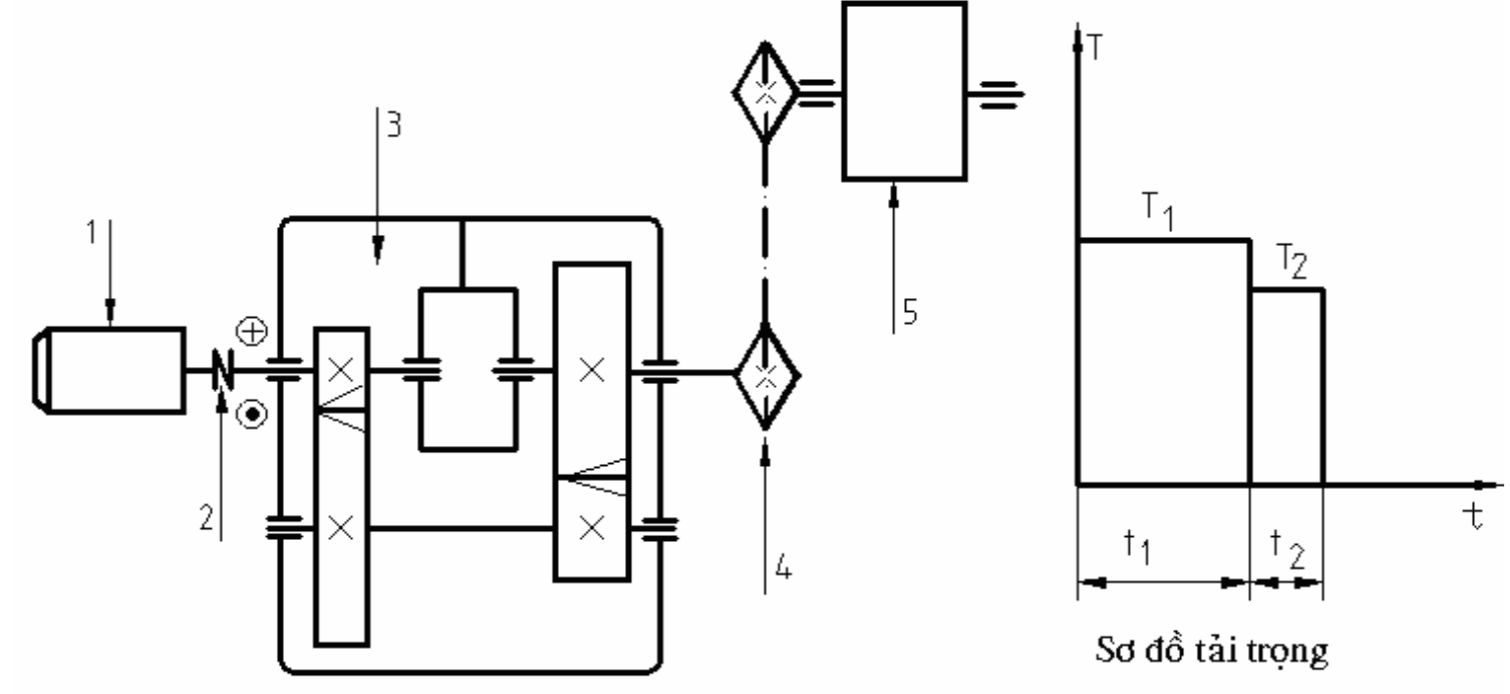
\includegraphics[width=\linewidth]{images/problem}
	\caption{Working principle diagram and workload of the mixing machine: 1) electric motor, 2) elastic coupling, 3) two-stage coaxial helical speed reducer, 4) roller chain drive, 5) mixing tank (one-directional, light duty, operate 1 shift, 8 hours each)}
	\label{fig:problem}
\end{figure}

\section{Mixing machine parameters}
From the parameters given in the document, we have:\\
\begin{tabular}{p{0.4\linewidth}p{0.4\linewidth}}
	$ P=7 \unitp{kW}$ & $ t_1=15\unitp{s} $\\
	$ n=65\unitp{rpm} $ & $ t_2=11\unitp{s} $\\
	$ L=8\unitp{years} $ & $ T_1=T\unitp{N\cdot m} $\\
	$ K_{ng}=260\unitp{days} $ & $ T_2=0.7T\unitp{N\cdot m} $\\
	$ Ca=1\unitp{shifts} $&\\
\end{tabular}

\section{Requirements}
\begin{itemize}
	\item 01 report.
	\item 01 assembly drawing.
	\item 01 detailed drawing.
\end{itemize}

\section{Design problem}
\begin{enumerate}
	\item Decide the working power of the electric motor and transmission ratio of the system.
	\item Calculate and design machine elements:
	\begin{enumerate}
		\item Calculate system drives (belt, chain or gear).
		\item Calculate the elements in speed reducers (gears, lead screws).
		\item Draw and calculate force diagram exerting on the transmission elements.
		\item Calculate, design shafts and keys.
		\item Choose bearings and couplings.
		\item Choose machine bodies, fasteners and other elements.
	\end{enumerate}
	\item Choose assembly tolerance.
	\item Bibliography
\end{enumerate}
%\begin{tabular}{p{0.5\linewidth}p{0.5\linewidth}}
%	\item 
%\end{tabular}
%\begin{table}[ht]
%	\centering
%	\begin{tabular}{lp{0.2\linewidth}p{0.12\linewidth}p{0.12\linewidth}p{0.12\linewidth}p{0.12\linewidth}p{0.12\linewidth}}\toprule
%		\multirow{2}{*}{} & \multirow{2}{*}{Sub functions} & \multicolumn{5}{l}{Solutions of the sub functions}\\\cmidrule{3-7}
%		& & 1 & 2 & 3 & 4 & 5\\
%		\midrule
%		A & Sub function 1 & \textbf{solution A1 (1) (3)} & solution A2 & solution A3 & &\\
%		B & Sub function 2 & solution B1 (1) (2) (3) & solution B2 (2) & \textbf{solution B3 (2)} & \multicolumn{2}{l}{solution B45} \\
%		C & Sub function 2 &  & solution C2 (2)  & \textbf{solution C3 (1)} & & solution C5 \\\bottomrule
%	\end{tabular}
%	\caption{A morphological box with 3 concept variants}
%\end{table}\\
%Legend\\
%(1) = thermal solution\\
%(2) = mechanical solution\\
%(3) = MEM solution

%For each bold option, if there are many concept variants, see Table \ref{subsub2}. In this example, we choose sub function B1 as the optimal solution with 3 variants. If the table does not describe fully or the sub function needs dividing into subgroups, see Table \ref{subsub1}.
%
%\begin{table}[ht]
%	\centering
%	\begin{tabular}{lp{0.2\linewidth}p{0.2\linewidth}p{0.2\linewidth}p{0.2\linewidth}}\toprule
%		\multirow{2}{*}{} & \multirow{2}{*}{Sub functions} & \multicolumn{3}{l}{Solutions of the sub functions}\\\cmidrule{3-5}
%		& & 1 & 2 & 3\\
%		\midrule
%		A & Sub function 1 & Thermal treatment & MEM treatment & \\
%		&  &   & MEM 1  & MEM 2 \\
%		B & ... &  &  &   \\\bottomrule
%	\end{tabular}
%	\caption{A morphological box with 3 concept variants}
%	\label{subsub1}
%\end{table}
%When calling a solution in Table \ref{subsub1}, we call it position + name of the sub solution (e.g. A2 MEM 1)
%\begin{table}[ht]
%	\centering
%	\begin{tabular}{lp{0.2\linewidth}p{0.2\linewidth}p{0.2\linewidth}p{0.2\linewidth}}\toprule
%		\multirow{2}{*}{} & \multirow{2}{*}{Sub functions} & \multicolumn{3}{l}{Solutions of the sub functions}\\\cmidrule{3-5}
%		& & 1 & 2 & 3\\
%		\midrule
%		B & Sub function 2 & & & \\
%		Ba & Type  &  Simple & Complex  & Mixed \\
%		Bb & Shape & Round & Square & Triangle  \\
%		Bc & Size $ \unitp{m} $  & 7x2 & 2x2 & 3x5 \\\bottomrule
%	\end{tabular}
%	\caption{A morphological box with 3 concept variants}
%	\label{subsub2}
%\end{table}
%
%\section{Evaluation Table}
%Many evaluation tables are developed in the industry (e.g VDI 2222, VDI 2225). Search for the sheet form on the internet, consult with your supervisor/customer for further information before using it.
%\begin{figure}[ht]
%	\centering
%	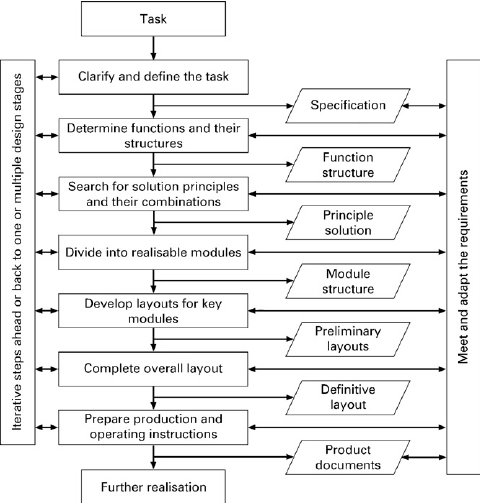
\includegraphics{images/01}
%	\caption{A figurative example of VDI 2222}
%	\label{fig:01}
%\end{figure}
%
%General points to remember to make better decisions:
%\begin{itemize}
%	\item Use consecutively (following one another).
%	\item Every table should have its own acronym since turning pages is avoided.
%	\item Simple points are related to almost other categories. Examples:\\
%	Parallel point values: load carrying $ \uparrow \Rightarrow $ beneficial $ \uparrow \Rightarrow $ simple point $ \uparrow $\\
%	Opposite point values: self-weight $ \uparrow \Rightarrow $ bad $ \downarrow \Rightarrow $ simple point $ \downarrow $
%	\item Think as a user/customer, not a manufacturer.
%\end{itemize}
%
%\section{Tabular Re-arrangement}
%Example:
%
%The sterilization temperature for sterilizing the tank should be at least $ 135\degc $ for $ 30 $ min. The sterilizing temperature at the condensomat should not fall below $ 125\degc $.
%
%You can "tabularize" the body of paragraph into a table, which is more concise and readable.\\\\
%\textbf{Minimum temperatures for sterilizing}
%\begin{table}[ht]
%	\begin{tabular}{p{0.4\textwidth}p{0.4\textwidth}}
%		\textbf{location} & \textbf{temperature}\\
%		at the tank & temp. $ =135\degc $, 30 min\\
%		at the condensomat & temp. $ =125\degc $
%	\end{tabular}
%\end{table}
%
%\section{Choosing between diagram, table and text descriptions}
%In general:
%\begin{itemize}
%	\item Text description is exact but hard to read.
%	\item Table is exact but still not easy to read.
%	\item Diagram is not exact but easy to visualize and memorable.
%	\item Placing the right thing on a page is essential for a great report.
%\end{itemize}
%The next important key point to remember is called text-figure-relationship, which is how and where you place texts and figures in a page:
%\begin{itemize}
%	\item Placing figures (diagrams and tables) in an appendix is good for positioning but leads to turning pages multiple times (bad text-figure-relationship).
%	\item Placing figures near/on the same page as the explaining text is a good text-figure-relationship. If the report is double-sided, the figure should be on the same double-page as the text (the diagram and explaining text should either be on odd or even pages).
%	\item Cross referencing to a figure with a statement and add the phrase "Figure xx." at the end after a comma.
%	\item Drawing/scanning the figures as early as possible while writing the explaining text.
%\end{itemize}
%
%Graphics simplify reality (e.g. principle drawing, map), explain abstract ideas by means of spatial arrangement (e.g. bar chart, pie chart, tree chart), create associations (e.g. logo and pictogram).
%
%There are 13 basic rules for information-effective design of figures:
%\begin{enumerate}
%	\item Accentuate important items.
%	\item Delete/leave out unimportant items (use max. 4-7 graphic elements in 1 picture or it is overloaded).
%	\item Line thickness and font size must be sufficient. Figures should be readable at a distance of 30-40 cm.
%	\item Relationship of graphic elements should be emphasized (lines, arrows, columns, rows, common color). These should be specified in detail (character of the relationship, meaning behind it) using labels and explanations in the legend.
%	\item Objects near each other belong together.
%	\item An element placed above or below other elements is regarded as hierarchically super-ordinate or sub-ordinate.
%	\item Logical/chronological sequence has its elements placed beside each other.
%	\item Circular arrangement is thought as a cycle or repeated sequence.
%	\item An element surrounding another element is understood as the outer includes the inner element.
%	\item Boxes, bars, lines, columns, etc. must be clearly marked (text labels or graphical explanations).
%	\item 1 type of element may have only 1 function within one/series of figures (e.g. arrows for vector direction).
%	\item $ x- $axis is horizontal, $ y- $axis is vertical
%	\item Look up for standardized symbols (e.g. DIN 66001 for flow charts, DIN 32520, DIN 66261).
%\end{enumerate}
%
%\chapter{Motor Design}
%\section{Nomenclature}
%\begin{tabular}[t]{lp{6cm}}
%	$ n_{bc} $ & rotational speed of belt conveyor, $ \unit{rpm} $\\
%	$ n_{sh} $ & rotational speed of shaft, $ \unit{rpm} $\\
%	$ P_m $ & maximum operating power of belt conveyor, $ \unit{kW} $\\
%	$ P_{motor} $ & calculated motor power to drive the system, $ \unit{kW} $\\
%	$ P_{sh} $ & operating power of shaft, $ \unit{kW} $\\
%	$ P_w $ & operating power of the belt conveyor given a workload, $ \unit{kW} $\\
%	$ u_{ch} $ & transmission ratio of chain drive\\
%\end{tabular}
%\begin{tabular}[t]{lp{6cm}}
%	$ u_{hg} $ & transmission ratio of helical gear\\
%	$ u_{sys} $ & transmission ratio of the system\\
%	$ T_{motor} $ & motor torque, $ \unit{N\cdot mm} $\\
%	$ T_{sh} $ & shaft torque, $ \unit{N\cdot mm} $\\
%	$ \delta_u $ & relative error of $ u_{sys} $\\
%	$ \eta_b $ & bearing efficiency\\
%	$ \eta_c $ & coupling efficiency\\
%	$ \eta_{ch} $ & chain drive efficiency\\
%	$ \eta_{hg} $ & helical gear efficiency\\
%	$ \eta_{sys} $ & efficiency of the system\\
%	$ _1 $ & shaft 1\\
%	$ _2 $ & shaft 2\\
%\end{tabular}
%
%\section{Calculate $ \eta_{sys} $}
%From table (2.3):\\
%$ \eta_c = 1 $\\
%$ \eta_b = 0.99 $\\
%$ \eta_{hg} = 0.96 $\\
%$ \eta_{ch} = 0.95 $\\
%$ \eta_{sys} = \eta_c\eta_b^3\eta_{hg}\eta_{ch} \approx 0.88 $
%
%\section{Calculate $ P_{motor} $}
%$ P_m = \dfrac{F_tv_{bc}}{1000} \approx 13.73 \unit{(kW)}$\\
%From equation (2.13) :\\
%$ P_w = P_m\sqrt{\dfrac{\left(\dfrac{T_1}{T}\right)^2t_1 + \left(\dfrac{T_2}{T}\right)^2t_2}{t_1+t_2}} \approx 10.41 \unit{(kW)} $\\
%$ P_{motor} = \dfrac{P_w}{\eta_{sys}} \approx 11.76\unit{(kW)} < P_m$
%
%\section{Calculate $ n_{motor} $}
%$ n_{bc} = \dfrac{6\times10^4v}{\pi D_{bc}} \approx 116.5 \unit{(rpm)}$\\
%$ u_{ch} = 5$ (table (2.4))\\
%$ u_{hg} = 5$ (table (2.4))\\
%$ u_{sys} = u_{ch}u_{hg} = 25 $\\
%$ n_{motor} = u_{sys}n_{bc} \approx 2912.54  \unit{(rpm)} $
%
%\section{Choose motor}
%To work normally, the maximum operating power of the chosen motor must be no smaller than both estimated $ P_{motor} $ and $ P_m $. Since $ P_{motor} < P_m $ for our case, the minimum operating power of choice is $ P_m $. In similar fashion, its rotational speed must also be no smaller than estimated $ n_{motor} $.\\
%Thus, from table (P1.3), we choose motor 4A160M2Y3 which operates at $ 18.5\unit{kW} $ and $ 2930\unit{rpm} $\\
%$\Rightarrow P_{motor} = 18.5\unit{kW}, n_{motor} = 2930\unit{(rpm)}$\\
%Recalculating $ u_{sys} $ with the new $ P_{motor} $ and $ n_{motor} $, we obtain:\\
%$ u_{sys} = \dfrac{n_{motor}}{n_{bc}} \approx 25.15	$\\
%Assuming $ u_{hg} = const $:\\
%$ u_{ch} = \dfrac{u_{sys}}{u_{hg}} \approx 5.03$
%\paragraph{Relative error of transmission ratio} The ratio is calculated as follows:
%\[\delta_u=\dfrac{|25.15-25|}{25} \approx 0.6\% \leq  5\%\]
%
%
%\section{Calculate power, rotational speed and torque}
%Let us denote $ P_{sh1} $, $ n_{sh1} $ and $ T_{sh1} $ be the transmitted power, rotational speed and torque onto shaft 1, respectively. Similarly, $ P_{sh2} $, $ n_{sh2} $ and $ T_{sh2} $ will be the transmitted parameters onto shaft 2. These notations will be used throughout the next chapters.
%\subsection{Power}
%$ P_{ch} = P_m \approx 13.73 \unit{(kW)}$\\
%$ P_{sh2} = \dfrac{P_{ch}}{\eta_b\eta_{ch}} \approx 14.59 \unit{(kW)}$\\
%$ P_{sh1} = \dfrac{P_{sh2}}{\eta_b\eta_{hg}} \approx 15.35 \unit{(kW)}$
%%$ P_{motor} = \dfrac{P_{sh1}}{\eta_c} \approx 15.35 \unit{(kW)}$
%\subsection{Rotational speed}
%$ n_{sh1} = n_{motor} = 2930\unit{(rpm)}$\\
%$ n_{sh2} = \dfrac{n_{sh1}}{u_{hg}} = 586 \unit{(rpm)}$
%\subsection{Torque}
%$ T_{motor} = 9.55\times10^6 \dfrac{P_{motor}}{n_{motor}} \approx 60298.63 \unit{(N\cdot mm)}$\\
%$ T_{sh1} = 9.55\times10^6 \dfrac{P_{sh1}}{n_{sh1}} \approx 50047.56 \unit{(N\cdot mm)}$\\
%$ T_{sh2} = 9.55\times10^6 \dfrac{P_{sh2}}{n_{sh2}} \approx 237825.99 \unit{(N\cdot mm)}$\\\\
%In summary, we obtain the following table:
%\begin{table}[ht]
%	\centering
%	\begin{tabular}{|
%			>{\columncolor[HTML]{C0C0C0}}l |l|l|l|l|}
%		\hline
%		& \multicolumn{1}{c|}{\cellcolor[HTML]{C0C0C0}Motor} & \multicolumn{2}{c|}{\cellcolor[HTML]{C0C0C0}Shaft 1} & \multicolumn{1}{c|}{\cellcolor[HTML]{C0C0C0}Shaft 2} \\ \hline
%		$ P \unit{(kW)}$ & 18.5                                            & \multicolumn{2}{l|}{15.35}                          & 14.59                                              \\ \hline
%		$ u $ & \multicolumn{2}{p{3.cm}|}{5}                                                         & \multicolumn{2}{l|}{5.03}                                                       \\ \hline
%		$ n \unit{(rpm)}$ & 2930                                               & \multicolumn{2}{l|}{2930}                            & 586                                                  \\ \hline
%		$ T \unit{(N\cdot mm)}$ & 60298.63  & \multicolumn{2}{l|}{50047.56}                      & 237825.99                                          \\ \hline
%	\end{tabular}
%	\caption{System overall specifications}
%\end{table}